\documentclass[12pt,openright,oneside,a4paper,english,french,spanish]{abntex2}

%%\usepackage{cmap}	
%%\usepackage{lmodern}	
%\usepackage[T1]{fontenc}	
%\usepackage[utf8]{inputenc}		
%\usepackage{lastpage}		
%\usepackage{indentfirst}
%\usepackage{color}	
%\usepackage{graphicx}	
%%\usepackage{units}
%\usepackage[brazilian,hyperpageref]{backref}
%\usepackage[alf]{abntex2cite}
%\usepackage{bold-extra}
%\usepackage{eso-pic}
%\usepackage{longtable}

\usepackage[pdftex]{color,graphicx}
\usepackage{cmap}	
\usepackage{lmodern}	
\usepackage[T1]{fontenc}	
\usepackage[utf8]{inputenc}		
\usepackage{lastpage}		
\usepackage{indentfirst}
\usepackage{color}	
\usepackage{graphicx}	
\usepackage{units}
\usepackage[brazilian,hyperpageref]{backref}
\usepackage[alf]{abntex2cite}
\usepackage{bold-extra}
\usepackage{eso-pic}
\usepackage{float}
\usepackage{longtable}
\usepackage[final]{pdfpages}
\usepackage{lscape}
\usepackage{mathtools}
\renewcommand{\backrefpagesname}{Citado na(s) página(s):~}
\renewcommand{\backref}{}
\renewcommand*{\backrefalt}[4]{
	\ifcase #1 %
		Nenhuma citação no texto.%
	\or
		Citado na página #2.%
	\else
		Citado #1 vezes nas páginas #2.%
	\fi}%
% ---


\newcommand{\curso}[1]{\def\imprimircurso{#1}}

\newcommand{\palavraChaveUm}[1]{\def\imprimirpalavrachaveum{#1}}
\newcommand{\palavraChaveDois}[1]{\def\imprimirpalavrachavedois{#1}}

\newcommand{\cdu}[1]{\def\nomecdu{#1}}
\newcommand{\dataDaAprovacao}[1]{\def\imprimirdatadaaprovacao{#1}}

\newcommand{\membroConvidadoUm}[1]{\def\imprimirmembroconvidadoum{#1}}
\newcommand{\membroConvidadoDois}[1]{\def\imprimirmembroconvidadodois{#1}}

\newcommand\BackgroundPic{%
	\put(0,0){%
		\parbox[b][\paperheight]{\paperwidth}{%
			\vfill
			\centering
			
\includegraphics[width=\paperwidth,height=\paperheight,%
				keepaspectratio]{figuras/capa.pdf}%
			\vfill
		}
	}
}

\renewcommand{\imprimircapa}{%
  \begin{capa}%
    \center
	\AddToShipoutPicture*{\BackgroundPic}

%	\begin{huge}
%		\textbf{\textsc{Trabalho de Conclusão de Curso}}
%	\end{huge}

    \vspace*{3.0in}
	{\textbf{\large\imprimirinstituicao}}
	\par
	{\textbf{\large\imprimircurso}}

	\vspace{2cm}

    {\ABNTEXchapterfont\bfseries\LARGE\imprimirtitulo}
    \vspace{2cm}
    
	\begin{flushright}
    	\textbf{{\large{Autor: \imprimirautor}}}
		\par
    	\textbf{{\large{Orientador: \imprimirorientador}}}
	\end{flushright}
		
    \vspace*{1cm}
    \textbf{{\large\imprimirlocal}}
    \par
    \textbf{{\large\imprimirdata}}
    
    \vspace{0.2in}
  \end{capa}
}



% Dados pessoais
\autor{Alana Gabriele Amorim Silva e Raquel Ferreira Andrade}
\curso{Engenharia de Software}

% Dados do trabalho
\titulo{SIGTCC: Sistema Integrado para Gestão e Acompanhamento de Trabalhos de Conclusão de Curso}
\data{2026}
\palavraChaveUm{autômatos celulares}
\palavraChaveDois{sistemas em chip}

% Dados da orientação
\orientador{Prof. Dr. Henrique Gomes de Moura}

% Dados para a ficha catalográfica
\cdu{-a definir-}

% Dados da aprovação do trabalho
\dataDaAprovacao{-}
\membroConvidadoUm{Prof. Dr. Carlos Humberto Llanos Quintero (ENM/FT/UnB)}
\membroConvidadoDois{Prof. Dr. Fabiano Araújo Soares (FGA/UnB)}
\local{Brasília, DF}
\instituicao{%
  Universidade de Brasília - UnB
  \par
  Faculdade do Gama - FGA
}
\tipotrabalho{Trabalho de Conclusão de Curso}
\preambulo{Monografia submetida ao curso de graduação em \imprimircurso\ da Universidade de Brasília, como requisito parcial para obtenção do Título 
de Bacharel em \imprimircurso.}

\definecolor{blue}{RGB}{41,5,195}
\makeatletter
\hypersetup{
     	%pagebackref=true,
		pdftitle={\@title}, 
		pdfauthor={\@author},
    	pdfsubject={\imprimirpreambulo},
	    pdfcreator={LaTeX with abnTeX2},
		pdfkeywords={abnt}{latex}{abntex}{abntex2}{trabalho acadêmico}, 
		colorlinks=true,       		% false: boxed links; true: colored links
    	linkcolor=blue,          	% color of internal links
    	citecolor=blue,        		% color of links to bibliography
    	filecolor=magenta,      		% color of file links
		urlcolor=blue,
		bookmarksdepth=4
}
\makeatother
\setlength{\parindent}{1.3cm}
\setlength{\parskip}{0.2cm}  
\makeindex


\usepackage{xcolor}
\usepackage{listings}

\usepackage{xcolor}% Farben
\usepackage{algorithm}% http://ctan.org/pkg/algorithms
\usepackage{algpseudocode}% http://ctan.org/pkg/algorithmicx
\usepackage{mdframed}% Hintergrundbox, Rahmen, ...

\definecolor{mGreen}{rgb}{0,0.6,0}
\definecolor{mGray}{rgb}{0.5,0.5,0.5}
\definecolor{mPurple}{rgb}{0.58,0,0.82}
\definecolor{backgroundColour}{rgb}{0.95,0.95,0.92}

\lstdefinestyle{CStyle}{
    backgroundcolor=\color{backgroundColour},   
    commentstyle=\color{mGreen},
    keywordstyle=\color{magenta},
    numberstyle=\tiny\color{mGray},
    stringstyle=\color{mPurple},
    basicstyle=\footnotesize,
    breakatwhitespace=false,         
    breaklines=true,                 
    captionpos=b,                    
    keepspaces=true,                 
    numbers=left,                    
    numbersep=5pt,                  
    showspaces=false,                
    showstringspaces=false,
    showtabs=false,                  
    tabsize=2,
    language=C
}

\begin{document}
\frenchspacing 
\imprimircapa
\imprimirfolhaderosto*

\begin{fichacatalografica}
	\vspace*{\fill}					% Posição vertical
	\hrule							% Linha horizontal
	\begin{center}					% Minipage Centralizado
	\begin{minipage}[c]{12.5cm}		% Largura
	
	\imprimirautor
	
	\hspace{0.5cm} \imprimirtitulo  / \imprimirautor. --
	\imprimirlocal, \imprimirdata-
	
	\hspace{0.5cm} \pageref{LastPage} p. : il. (algumas color.) ; 30 cm.\\
	
	\hspace{0.5cm} \imprimirorientadorRotulo~\imprimirorientador\\
	
	\hspace{0.5cm}
	\parbox[t]{\textwidth}{\imprimirtipotrabalho~--~\imprimirinstituicao,
	\imprimirdata.}\\
	
	\hspace{0.5cm}
		1. \imprimirpalavrachaveum.
		2. \imprimirpalavrachavedois.
		I. \imprimirorientador.
		II. Universidade de Brasília.
		III. Faculdade do Gama.
		IV. \imprimirtitulo\\ 			
	
	\hspace{8.75cm} CDU \nomecdu\\
	
	\end{minipage}
	\end{center}
	\hrule
\end{fichacatalografica}

\input{editaveis/errata}
\begin{folhadeaprovacao}

  \begin{center}
    {\ABNTEXchapterfont\large\imprimirautor}

    \vspace*{\fill}\vspace*{\fill}
    {\ABNTEXchapterfont\bfseries\Large\imprimirtitulo}
    \vspace*{\fill}
    
    \hspace{.45\textwidth}
    \begin{minipage}{.5\textwidth}
        \imprimirpreambulo
    \end{minipage}%
    \vspace*{\fill}
   \end{center}
    
   Trabalho aprovado. \imprimirlocal, \imprimirdatadaaprovacao:

   \assinatura{\textbf{\imprimirorientador} \\ Orientador} 
   \assinatura{\textbf{\imprimirmembroconvidadoum} \\ Convidado 1}
   \assinatura{\textbf{\imprimirmembroconvidadodois} \\ Convidado 2}
      
   \begin{center}
    \vspace*{0.5cm}
    {\large\imprimirlocal}
    \par
    {\large\imprimirdata}
    \vspace*{1cm}
  \end{center}
  
\end{folhadeaprovacao}

\begin{dedicatoria}
   \vspace*{\fill}
   \centering
   \noindent
   \textit{Dedico este trabalho à minha amada família.} \vspace*{\fill}
\end{dedicatoria}

%\begin{agradecimentos}
\textbf{Caso não deseje utilizar os agradecimentos, deixar toda este arquivo
em branco}.
\end{agradecimentos}

%\begin{epigrafe}
    \vspace*{\fill}
	\begin{flushright}
		\textbf{A epígrafe é opcional. Caso não deseje uma, deixe todo
		este arquivo em branco}.

		\textit{``Não vos amoldeis às estruturas deste mundo, \\
		mas transformai-vos pela renovação da mente, \\
		a fim de distinguir qual é a vontade de Deus: \\
		o que é bom, o que Lhe é agradável, o que é perfeito.\\
		(Bíblia Sagrada, Romanos 12, 2)}
	\end{flushright}
\end{epigrafe}

\begin{resumo}

Os organismos artificiais celulares são circuitos que encapsulam e controlam arquiteturas integradoras, capacitadas para a execução de todos os cálculos requeridos sobre o domínio discreto escolhido. Os autômatos celulares constituem uma alternativa para modelagem de sistemas físicos em domínio discreto. Neste trabalho, o fenômeno físico considerado como estudo de caso é a propagação de ondas sonoras através de um meio ideal e estacionário. O trabalho foi realizado em duas etapas, sendo a primeira voltada para ao desenvolvimento de um sistema celular autômato (CA) aplicável à emulação de ondas planas unidimensionais, para aplicação em circuitos reconfiguráveis, e a segunda voltada para a apresentação de propostas de implementação em chip. O sistema CA desenvolvido, denominado Camphs1D, é composto de duas células autômatas, baseadas em IP-cores de operadores aritméticos em 27 bits, capazes de operar todos os fenômenos básicos de onda em meios unidimensionais. As mencionadas células foram desenvolvidas a partir de duas estratégias distintas, sendo a primeira descrita diretamente em VHDL, no software Vivado, e a segunda descrita em C/C++, no software Vivado HLS, onde foram usados IP-cores de ponto flutuante de 32 bits da Xilinx. Foram utilizadas, para efeito de validação de resultados, simulações em \textit{Testbench} VHDL, simulações no software SDK (Xilinx), e implementações físicas integradas com um processador ARM, para acesso à memória DDR disponível em placa. Todas as validações atingiram seus objetivos, relacionados à comparações com os mesmos resultados obtidos por modelos de referência, desenvolvidos a partir da solução de d'Alembert para a equação unidimensional da onda.

 \vspace{\onelineskip}
    
 \noindent
 \textbf{Palavras-chaves}: autômatos celulares; malha de guias digitais de ondas; sistemas em chip.
\end{resumo}

\begin{resumo}[Abstract]
 \begin{otherlanguage*}{english}
  
 Artificial cellular organisms are circuits able to encapsulate and control integrative architectures, capable of performing all required calculations on the chosen discrete domain. Cellular automata are an alternative for modeling physical systems in a discrete domain. In this work, the physical phenomenon considered, as a case study, is the sound wave propagation through an ideal and stationary medium. The work was carried out in two stages, the first focused on the development of a CA system, applied to one-dimensional plane wave propagation, in a reconfigurable circuitry, and the second focused on its on-chip implementation proposals. The developed CA system, called Camphs1D, is composed of two automata cells, based on IP-cores of 27-bit arithmetic operators, capable of operate all basic wave phenomena in one-dimensional media. The aforementioned cells were developed from two different strategies, the first one directly described in VHDL, using Vivado software, and the second one using C/C++, using Vivado HLS software, where Xilinx 32-bit floating point IP-cores were used. In order to validate results, simulations were used in Testbench VHDL, simulations in SDK software (Xilinxs), and physical implementations integrated with a software ARM terminator and DDR memory access. All validations achieved their goals, when compared with the reference models, developed from the solution of d'Alembert for the one-dimensional wave equation.
 
 \vspace{\onelineskip}
 
 \noindent 
 \textbf{Key-words}: cellular automaton; digital waveguide mesh; systems on chip.
 \end{otherlanguage*}
\end{resumo}

\pdfbookmark[0]{\listfigurename}{lof}
\listoffigures*
\cleardoublepage
\pdfbookmark[0]{\listtablename}{lot}
\listoftables*
\cleardoublepage

\begin{siglas}
  \item [TCC] Trabalho de Conclusão de Curso
  \item [ABNT] Associação Brasileira de Normas Técnicas
  \item [BDM] Biblioteca Digital de Monografias  
  \item [LGPD] Lei Geral de Proteção de Dados Pessoais
  \item [FCTE] Faculdade de Ciências e Tecnologias em Engenharia - Campus UnB Gama
  

\end{siglas}

%\begin{simbolos}
  \item[$ \Gamma $] Letra grega Gama
  \item[$ \Lambda $] Lambda
  \item[$ \zeta $] Letra grega minúscula zeta
  \item[$ \in $] Pertence
\end{simbolos}

\pdfbookmark[0]{\contentsname}{toc}
\tableofcontents*
\cleardoublepage


\textual

\chapter[Introdução]{Introdução}

\section{Contextualização}

O Trabalho de Conclusão de Curso (TCC) consiste em um trabalho acadêmico desenvolvido ao final de uma formação. De acordo com a Associação Brasileira de Normas Técnicas (ABNT), por meio da NBR 14724, o TCC é um documento que representa o resultado de um estudo, no qual o estudante deve expressar conhecimento do assunto escolhido, obrigatoriamente vinculado à disciplina, módulo, curso ou programa, e elaborado sob a coordenação de
um orientador \cite{ABNT2024}.

% O desenvolvimento do TCC envolve diferentes etapas e a participação de estudantes, orientadores e da instituição de ensino. O acompanhamento do cronograma e a interação entre orientador e orientando constituem aspectos desse processo, conforme discutido por \citeonline{Viana2010}.

% A relação entre orientador e orientando pode apresentar
% dificuldades ao longo do desenvolvimento do trabalho.
% \citeonline{Viana2010} destacam que o cumprimento do
% cronograma é uma responsabilidade compartilhada entre
% ambos, envolvendo a realização das atividades previstas
% e o acompanhamento das orientações. Entretanto, as autoras
% identificam dificuldades nesse processo, como a necessidade
% de alguns orientadores buscarem contato com seus orientandos e a sobrecarga de trabalho de determinados docentes, que pode comprometer a disponibilidade para o atendimento. De maneira semelhante, \citeonline{LeiteFilho2006} apontam a falta de contato entre orientador e orientando como uma das principais dificuldades dessa relação, frequentemente associada à falta de tempo dos envolvidos.

% Na Faculdade de Ciências e Tecnologias em Engenharia (FCTE) da Universidade de Brasília (UnB), o TCC é regulamentado pela Resolução do Conselho da FCTE nº 0002/2022, que estabelece sua organização em dois componentes curriculares. O TCC 1 possui caráter qualificatório, com o objetivo de avaliar a aptidão e a maturidade do discente e do tema em sua área de investigação. Já o TCC 2 corresponde à versão definitiva do trabalho, destinada à sua apresentação e validação. Ambos os componentes são avaliados por bancas examinadoras específicas.
% Após a avaliação, o resultado é registrado em ata e, no caso do
% TCC 2 aprovado, a versão definitiva é encaminhada para
% disponibilização na Biblioteca Digital de Monografias (BDM)
% \cite{UnB2022}.

A orientação acadêmica constitui uma parte importante do desenvolvimento do trabalho e pode apresentar dificuldades ao longo desse processo.\citeonline{Viana2010} descrevem a orientação acadêmica como uma relação pedagógica estabelecida entre orientador e orientando e apontam a existência de contribuições e fragilidades relacionadas a ambos os envolvidos. As autoras destacam que, por se tratar de uma relação dinâmica entre indivíduos com diferentes características pessoais e profissionais, essa interação pode se estabelecer de maneiras distintas, o que reforça a importância do diálogo entre as partes na construção do trabalho acadêmico.

Além do diálogo estabelecido durante a orientação, o acompanhamento do cronograma e a participação nas etapas também fazem parte desse processo. \citeonline{Viana2010} destacam que o cumprimento do cronograma é uma responsabilidade compartilhada entre orientador e orientando. As autoras identificam, entretanto, dificuldades nesse acompanhamento, tanto pela necessidade de alguns orientadores buscarem ativamente seus orientandos quanto pela sobrecarga de trabalho de alguns docentes, que pode comprometer o atendimento aos alunos. Semelhantemente, \citeonline{LeiteFilho2006} apontam a ausência de contato, decorrente da falta de tempo de ambas as partes, como o principal fator que dificulta a relação, e observam que a frequência dos encontros costuma depender da iniciativa do orientando.

% Além do orientador e do orientando, a coordenação também faz parte do processo, aprovando a composição das bancas, acompanhando o andamento dos trabalhos, controlando os prazos e reunindo as atas e menções ao final de cada semestre. Embora o regulamento da FCTE faça referência a um sistema eletrônico próprio para a matrícula nos componentes, a divulgação de menções, o registro das atas e a emissão de comprovante de participação ou orientação de banca, esses sistemas se limitam a etapas administrativas pontuais e não acompanham o trabalho enquanto ele está sendo desenvolvido. Nesse sentido, reuniões, comentários sobre versões do texto e ajustes de cronograma costumam ser registrados em diferentes meios de comunicação, como email e aplicativos de mensagem, sem um histórico centralizado que permita aos envolvidos acompanhar o progresso do trabalho.

% Dessa forma, o desenvolvimento do TCC envolve diferentes atividades, etapas e participantes, não se restringindo apenas à elaboração do trabalho acadêmico. O processo demanda acompanhamento ao longo de sua realização e envolve a interação entre estudantes, orientadores e a própria instituição de ensino. Nesse contexto,  Assim, este trabalho tem como foco a organização e o acompanhamento das diferentes etapas que compõem o ciclo de vida do TCC.

Dessa forma, o desenvolvimento do TCC não se restringe à elaboração do documento acadêmico. O processo demanda acompanhamento ao longo de sua realização e envolve a interação entre estudantes, orientadores e a própria instituição de ensino. Nesse contexto, este trabalho tem como foco a gestão e o acompanhamento do ciclo de vida do Trabalho de Conclusão de Curso.


\section{Justificativa}

O uso de tecnologias digitais tem se tornado cada vez mais presente no ambiente acadêmico, especialmente a partir das transformações ocorridas durante a pandemia de COVID-19. Mesmo após o retorno das atividades presenciais, práticas digitais incorporadas nesse período permaneceram presentes no ensino superior, sendo utilizadas em diferentes atividades acadêmicas e profissionais \cite{Carneiro2026}.

Nesse contexto, a utilização de ambientes virtuais passou a envolver não apenas o acesso a conteúdos, mas também atividades relacionadas à organização, à gestão de tarefas e ao acompanhamento das interações acadêmicas  \cite{Carneiro2026}. Essa realidade demonstra a aplicação dos recursos digitais no suporte a diferentes processos acadêmicos, criando possibilidades para sua utilização também na organização e no acompanhamento de atividades que envolvem diferentes etapas e participantes.

Nesse panorama, o processo de elaboração do TCC apresenta características que favorecem a utilização desse suporte. Visto que envolve etapas sequenciais, prazos definidos, entregas intermediárias e a participação de diferentes atores, seu acompanhamento depende da organização e atualização de informações que, atualmente, permanecem dispersas. Nesse sentido, a centralização dessas informações em um único ambiente pode contribuir para uma visão mais organizada do processo, facilitando o acompanhamento das etapas e das responsabilidades de cada um dos envolvidos.

% Apesar da existência de ferramentas voltadas para etapas específicas da gestão do TCC, o processo de desenvolvimento envolve informações e tarefas que vão além desses registros pontuais. A escolha do orientador, o planejamento das atividades, o acompanhamento de prazos, o registro de reuniões, o compartilhamento de documentos e o controle das entregas frequentemente ocorrem de maneira descentralizada. 

Diante desse cenário, faz-se necessária uma solução digital voltada especificamente para o acompanhamento do ciclo de vida do TCC. Um ambiente centralizado pode reunir informações relacionadas ao trabalho, como o andamento das etapas, os registros das reuniões e os documentos produzidos ao longo do processo, facilitando a comunicação entre o estudante e o orientador e oferecendo à coordenação uma visão ampla dos trabalhos em andamento e de suas respectivas situações.

% Dado o exposto, a escolha deste tema justifica-se pela necessidade de tornar o processo de desenvolvimento e acompanhamento dos trabalhos de Conclusão de Curso mais organizado, integrado e acessível aos envolvidos. A existência de informações, atividades e documentos distribuídos em diferentes meios pode dificultar tanto o acompanhamento realizado por alunos e orientadores quanto a visão da coordenação sobre o andamento dos trabalhos. Portanto, o desenvolvimento de um sistema voltado especificamente para esse contexto apresenta-se como uma oportunidade de reunir, em um único ambiente, recursos que auxiliem na organização das etapas, no acompanhamento de prazos e atividades, no registro das interações e na gestão das informações produzidas ao longo do TCC. Assim, a escolha pelo desenvolvimento dessa solução busca contribuir para uma gestão melhor estruturada do processo, atendendo às necessidades identificadas ao longo do ciclo de vida do Trabalho de Conclusão de Curso.


\section{Questão da Pesquisa}

Diante das dificuldades encontradas, este trabalho busca responder à seguinte questão:

\textbf{Como um sistema integrado pode contribuir para a gestão e o acompanhamento do ciclo de vida do Trabalho de Conclusão de Curso, considerando as necessidades de alunos, orientadores e coordenação?}

Nesse contexto, propõe-se o desenvolvimento de uma aplicação web que facilite a gestão e o acompanhamento das etapas do TCC, considerando as necessidades dos envolvidos.

\section{Objetivos}

Esta seção apresenta o objetivo geral e os objetivos específicos deste trabalho.

\subsection{Objetivo Geral}

Desenvolver uma aplicação web que centralize e facilite a gestão e o acompanhamento do ciclo de vida do TCC, atendendo às necessidades de alunos, orientadores e coordenação.

\subsection{Objetivos Específicos}

Os objetivos específicos descrevem as etapas necessárias para o desenvolvimento da solução proposta, considerando as necessidades dos usuários, os requisitos do sistema e as práticas de Engenharia de Software adotadas ao longo do projeto. Nesse sentido, foram definidos os seguintes objetivos específicos:

\begin{enumerate}
    \item Levantar as necessidades e dificuldades de estudantes, orientadores e coordenação no processo de TCC por meio da aplicação de questionários.
    \item Identificar e definir os requisitos do sistema a partir das necessidades levantadas.
    \item Projetar a interface e os fluxos de interação do sistema.
    \item Desenvolver a interface web responsiva do sistema.
    \item Desenvolver a API responsável pelas regras de negócio e pela comunicação entre os componentes da aplicação.
    \item Implementar o armazenamento e o gerenciamento dos dados da aplicação.
    \item Avaliar a solução desenvolvida com os usuários envolvidos no processo de TCC.
\end{enumerate}

Os objetivos específicos foram divididos em duas etapas, sendo os quatro primeiros realizados na primeira entrega deste trabalho, enquanto os objetivos de 5 a 7 serão desenvolvidos na segunda etapa.


\section{Organização da Monografia}



\section{Uso de Inteligência Artificial}

Durante a realização deste trabalho, ferramentas de Inteligência Artificial (IA) serão utilizadas como apoio à elaboração do documento acadêmico e ao desenvolvimento da aplicação. Na produção textual, seu uso será direcionado à revisão ortográfica e à melhoria da clareza e organização do texto. 

No desenvolvimento da aplicação, a IA será utilizada na construção da interface web, incluindo a geração e o aprimoramento de componentes e funcionalidades do frontend. O código produzido será revisado e validado pelos autores, que permanecerão responsáveis pelas decisões técnicas e pela implementação da solução.
\chapter[Referencial Teórico]{Referencial Teórico}

\section{Trabalho de Conclusão de Curso}

O Trabalho de Conclusão de Curso desempenha um papel
importante na formação acadêmica, proporcionando ao
estudante a oportunidade de desenvolver atividades de
pesquisa e aplicar conhecimentos adquiridos durante a
graduação. Segundo \citeonline{Trindade2018}, o TCC
pode contribuir para a formação de profissionais com
maior capacidade crítica e reflexiva, ao estimular a
investigação e a construção do conhecimento.

Além da produção acadêmica, o desenvolvimento do TCC
está relacionado à autonomia do estudante.
\citeonline{Trindade2018} destacam que a realização
de atividades de pesquisa favorece o desenvolvimento
da iniciativa e da capacidade de analisar questões
de maneira crítica, competências que também podem
contribuir para a atuação profissional.

Os autores também ressaltam que o TCC não precisa
necessariamente apresentar uma descoberta inédita,
podendo abordar assuntos relacionados à área de
formação do estudante. Nesse sentido, sua relevância
não está apenas no resultado apresentado, mas também
nas experiências de aprendizagem proporcionadas
durante sua elaboração.


\subsection{Organização do TCC na FCTE}

Na Faculdade de Ciências e Tecnologias em Engenharia (FCTE)
da Universidade de Brasília (UnB), o Trabalho de Conclusão
de Curso é regulamentado pela Resolução do Conselho da FGA
nº 0002/2022, que estabelece sua organização em dois
componentes curriculares: TCC 1 e TCC 2 \cite{UnB2022}.

O TCC 1 possui caráter qualificatório, tendo como objetivo
avaliar a aptidão e a maturidade do discente e do tema
escolhido em sua área de investigação. Já o TCC 2 corresponde à versão definitiva do trabalho, destinada à sua apresentação e validação. Ambos os componentes são avaliados por bancas examinadoras específicas \cite{UnB2022}.

Após a avaliação, o resultado é registrado em ata e, no caso do TCC 2 aprovado, a versão definitiva é encaminhada para disponibilização na Biblioteca Digital de Monografias (BDM) \cite{UnB2022}.

Além das atividades realizadas pelos estudantes e orientadores, a coordenação também participa dos procedimentos acadêmicos
relacionados ao TCC, incluindo a aprovação da composição das bancas, o acompanhamento dos trabalhos, o controle dos prazos e a reunião das atas e menções ao final de cada semestre \cite{UnB2022}.

\section{Sistemas de Informação no Ensino Superior}

\subsection{Sistemas de Informação na Gestão Acadêmica}

\section{Trabalhos e Soluções Relacionadas}

\section{Análise e Discussão}
\chapter[Referencial Tecnológico]{Referencial Tecnológico}

Este capítulo apresenta as principais ferramentas e tecnologias utilizadas na realização deste trabalho. Para melhor organização, elas foram agrupadas de acordo com sua finalidade no projeto, contemplando recursos de apoio à produção acadêmica e à pesquisa, prototipação, desenvolvimento da aplicação, armazenamento de dados e ferramentas auxiliares.

A Figura \ref{fig:nuvem-tecnologias} apresenta uma nuvem de palavras com as principais tecnologias e ferramentas previstas para este trabalho. O tamanho de cada termo representa o grau de responsabilidade esperado da tecnologia no desenvolvimento do projeto, enquanto as cores indicam sua finalidade: azul para tecnologias centrais, verde para tecnologias complementares, roxo para infraestrutura e cinza para ferramentas auxiliares. Essa classificação foi definida pelos autores com base na participação prevista de cada tecnologia na solução proposta.

\begin{figure}[htbp]
    \centering
    
\includegraphics[width=0.85\textwidth]{figuras/nuvem-tecnologica.png}
    \caption{Nuvem de palavras das tecnologias previstas para o projeto}
    \label{fig:nuvem-tecnologias}
    \fonte{Elaboração própria (2026).}
\end{figure}


\section{Ferramentas de Apoio à Produção Acadêmica e à Pesquisa}

A elaboração deste documento foi realizada em \textbf{LaTeX}, um sistema de preparação de documentos utilizado na produção de textos técnicos e científicos, que permite estruturar elementos como capítulos, figuras, tabelas e referências bibliográficas de maneira padronizada. A edição foi feita por meio do \textbf{Overleaf}, uma plataforma online para criação e compilação de documentos LaTeX no navegador, dispensando a configuração de um ambiente local.

Para o levantamento de requisitos, será utilizado o \textbf{Google Forms}, ferramenta online para criação e aplicação de formulários e questionários. Por intermédio dela serão coletadas informações sobre as necessidades e dificuldades de estudantes, orientadores e coordenação no processo de TCC, cujos resultados auxiliarão na definição dos requisitos do sistema.

O \textbf{Canva} e o \textbf{GIMP} são ferramentas utilizadas para criação e edição de elementos visuais. O Canva é uma plataforma online de design gráfico, enquanto o GIMP é um software livre de edição e manipulação de imagens. Neste trabalho, ambas as ferramentas serão utilizadas na elaboração e edição de diagramas, figuras e outros elementos visuais que compõem o documento acadêmico.

\section{Prototipação e Desenvolvimento da Aplicação}

Antes da implementação definitiva, será desenvolvido um protótipo de alta fidelidade das telas e dos fluxos de interação do sistema, utilizando as mesmas tecnologias previstas para a aplicação final. Essa abordagem permite obter uma representação navegável e próxima do produto real, possibilitando a validação das interfaces junto aos usuários antes da implementação completa das funcionalidades, além de permitir o reaproveitamento de parte do código gerado durante a prototipação. 

A aplicação será desenvolvida em \textbf{TypeScript}, linguagem baseada em JavaScript que acrescenta recursos de tipagem estática. A utilização será utilizado tanto no frontend quanto no backend, contribuindo para a padronização do desenvolvimento e para a definição das estruturas de dados utilizadas pela aplicação. 

No frontend, será utilizado o \textbf{React}, biblioteca JavaScript que permite construir interfaces por meio de componentes reutilizáveis. A biblioteca utiliza JSX, uma extensão de sintaxe que possibilita escrever estruturas semelhantes ao HTML junto à lógica dos componentes. A estilização será realizada com o \textbf{Tailwind CSS}, framework baseado em classes utilitárias que facilita a implementação de interfaces responsivas.

No backend, será utilizado o \textbf{Node.js}, ambiente de execução JavaScript utilizado, entre outras finalidades, no desenvolvimento de aplicações no lado do servidor, em conjunto com o \textbf{NestJS}, framework que oferece suporte nativo ao TypeScript e uma estrutura modular para a organização do código. A partir dessas tecnologias serão implementadas a API REST e as regras de negócio do sistema.

\section{Armazenamento de Dados e Apoio ao Desenvolvimento}

Os dados da aplicação serão armazenados no \textbf{PostgreSQL}, sistema gerenciador de banco de dados relacional. O \textbf{Prisma ORM} será responsável pela comunicação entre o backend e o banco de dados, permitindo realizar operações de consulta e manipulação das informações armazenadas.

O editor de código-fonte \textbf{Visual Studio Code} será utilizado como ambiente principal para o desenvolvimento do frontend e do backend da aplicação. Os endpoints disponibilizados pela API serão testados com o 
\textbf{Postman}, ferramenta utilizada para desenvolvimento e teste de APIs. Por fim, o \textbf{Docker} será usado para executar a aplicação e seus serviços em contêineres, padronizando o ambiente de execução dos componentes do sistema e facilitando sua configuração durante o desenvolvimento.


% \chapter[Resultados]{Resultados}

Este capítulo se inicia com os resultados das simulações comportamentais realizadas sobre os organismos artificiais Camphs1D05G1 e Camphs1DB9G2. Outros detalhes do projeto das arquiteturas mencionadas, tais como geradores de código e conversores numéricos, também serão apresentados. Em seguida, serão apresentados os relatório de consumo, bem como os resultados obtidos a partir das implementações realizadas em placa.

\section{Simulações comportamentais}

\subsection{Organismo artificial Camphs1D05G1}

Os resultados desta primeira simulação foram úteis para a validação de todas as funcionalidades do sistema CA desenvolvido. As figuras seguintes trazem imagens obtidas da simulação comportamental realizada no software VIVADO, para os sinais de controle apresentados no capítulo anterior.

\begin{figure}[h]
	\centering
	\label{sim1.png}
		\includegraphics[keepaspectratio=true,scale=0.48]{figuras/sim1.png}
	\caption{\label{fig:padrao}Simulação comportamental da organismo artificial Camphs1D05G1. Em tela, um visão geral das variáveis envolvidas.}
\end{figure}

Um sinal impulsivo foi gerado pela célula GCA1D central. Após mudança de valor do sinal MODE, conectado à esta célula, esta célula autômata passou a operar apenas com a dispersão das ondas transmitidas.

É possível observar na Figura \ref{fig:padrao} um padrão de resposta que se repete com o tempo, na Figura dos sinais s\_left\_stim\_* e s\_right\_stim\_*. Estes sinais representam os estímulos de saída de ondas nas células autômatas. Este comportamento é desejado devido às sucessivas reflexões de ondas geradas pelas células HCA1D posicionadas nos extremos do sistema.

Na Figura \ref{fig:china}, a seguir, serão apresentados os primeiros eventos esperados para este sistema CA, em acordo com o modelo de referência (no que tange o fenômeno observado).

\begin{figure}[h]
	\centering
	\label{camphs1d1_exp.png}
		\includegraphics[keepaspectratio=true,scale=0.7]{figuras/camphs1d1_exp.png}
	\caption{\label{fig:china}Resultados esperados para o sistema Camphs1D05G1, com base nos fenômenos básicos da onda. Cada linha apresentada representa as saídas da equação de d'Alembert, submetida ao sinal de entrada (célula 3), em cada um dos 5 nós da solução discreta. Temos também representadas as duas direções de movimento das ondas acústicas.}
\end{figure}

O coeficientes internos às células HCA1D foram ajustados para emularem um coeficiente de reflexão  $r=0.5$. O padrão repetido visto na Figura \ref{fig:padrao} fica agora mais fácil de ser compreendido, pois percebemos que as ondas sonoras devem, gradualmente, perder $50\%$ das suas amplitudes a cada reflexão.

\begin{figure}[h]
	\centering
	\label{sim2.png}
		\includegraphics[keepaspectratio=true,scale=0.6]{figuras/sim2.png}
	\caption{\label{fig:sequencia}Resultado esperado para o sistema Camphs1D05G1, com base nos fenômenos básicos da onda. Em tela, temos os sinais de estímulo gerados.}
\end{figure}

Na Figura \ref{fig:sequencia} podemos comprovar a sequência de geração de estímulos esperada - é possível verificá-la na Figura \ref{fig:china}. Primeiramente a célula 3 (fonte) gera estímulos nas duas direções, com amplitude igual a 200. Em seguida, a célula 4 gera um estímulo para a sua célula a direita (s\_left\_stim\_4), juntamente com as células 2, que gera um estímulo para a sua vizinha à esquerda (s\_right\_stim\_2). Neste mesmo ciclo, a célula 3 gera novamente seus estímulos bidirecionais, desta vez para o valor 0. Deste modo, a simulação prossegue, atendendo perfeitamente às expectativas para com a solução.

\begin{figure}[h]
	\centering
	\label{sim3.png}
		\includegraphics[keepaspectratio=true,scale=0.68]{figuras/sim3.png}
	\caption{\label{fig:valores1}Resultado esperado para o sistema Camphs1D05G1, com base nos fenômenos básicos da onda. Em tela, as amplitudes de onda transmitidas pelas células autômatas.}
\end{figure}

Na Figura \ref{fig:valores1} observamos as amplitudes das ondas transmitidas pelas células autômatas, em acordo com os estímulos gerados pelas suas vizinhas. Os valores em hexadecimais $21a4000_h$, $2164000_h$ e $2124000_h$ representam os decimais $200_d$, $100_d$ e $50_d$, respectivamente.

Para finalizar esta exposição, é possível checar as saídas dos canais receptores posicionados na célula 2, e sequência observada coincide perfeitamente com o padrão esperado. Os resultados podem ser apreciados na Tabela \ref{tab:cinco}, a seguir. 

Cada ciclo do sistema CA, indicado na Tabela \ref{tab:cinco}, corresponde a um intervalo de 4 ciclos de relógio. Os ciclos de 1 a 9 correspondem exatamente com os resultados apresentados na Figura \ref{fig:china}, e foram contabilizados a partir do primeiro sinal de START.

\begin{table}
\centering
\caption{\label{tab:cinco} Valores registrados nos canais de saída de Camphs1D05G1.}
\begin{tabular}{ |p{3cm}|p{3cm}|p{3cm}| }
 \hline
 \multicolumn{3}{|c|}{S\_LEFT\_OUT} \\
 \hline \hline
Ciclo & Valor Obtido & Valor esperado \\
 \hline
 1 & 0000000_h & 0000000_h \\
 2 & 0000000_h & 0000000_h \\
 3 & 0000000_h & 0000000_h \\
 4 & 2164000_h & 2164000_h \\
 5 & 0000000_h & 0000000_h \\
 6 & 0000000_h & 0000000_h \\
 7 & 0000000_h & 0000000_h \\
 8 & 2124000_h & 2124000_h \\
 9 & 0000000_h & 0000000_h \\
 10 & 0000000_h & 0000000_h \\
 11 & 0000000_h & 0000000_h \\
 \hline
 \multicolumn{3}{|c|}{S\_RIGHT\_OUT} \\
 \hline \hline
Ciclo & Valor Obtido & Valor esperado \\
 \hline
 1 & 0000000_h & 0000000_h \\
 2 & 21a4000_h & 21a4000_h \\
 3 & 0000000_h & 0000000_h \\
 4 & 0000000_h & 0000000_h \\
 5 & 0000000_h & 0000000_h \\
 6 & 2164000_h & 2164000_h \\
 7 & 0000000_h & 0000000_h \\
 8 & 0000000_h & 0000000_h \\
 9 & 0000000_h & 0000000_h \\
 10 & 2124000_h & 2124000_h \\
 11 & 0000000_h & 0000000_h \\
 \hline
\end{tabular}
\end{table}

\subsection{Dados de entrada, saída e decodificações realizadas em Camphs1D05G1}

Serão apresentados aqui apenas os conteúdos dos arquivos utilizados para a introdução dos sinais de controle. O procedimento de saída de valores, nos canais receptores, também será discutido.

O organismo artificial Camphs1D05G1 foi projetado para executar a leitura de 3 arquivos de dados: sce\_value.txt, sce\_start.txt e sce\_modes.txt. Os arquivos são lidos nas bordas de subida do relógio - o sinal de RESET foi acionado na primeira borda de subida do relógio para inicializar todos os registradores internos. O conteúdos dos arquivos estão apresentados na Tabela \ref{tab:arquivos1}.

\begin{table}
\centering
\caption{\label{tab:arquivos1} Conteúdo dos arquivos de controle utilizados na simulação comportamental do organismo artificial Camphs1D05G1.}
\begin{tabular}{ |p{3cm}|p{3cm}|p{6cm}| }
 \hline
 \multicolumn{3}{|c|}{Linhas dos Arquivos de Controle} \\
 \hline \hline
sce_modes.txt & sce_start.txt & sce_value.txt \\
 \hline
 10_b & 0_b & 010000010010000000000000000_b \\
 10_b & 0_b & 010000010010000000000000000_b \\
 10_b & 1_b & 010000010010000000000000000_b \\
 10_b & 0_b & 010000010010000000000000000_b \\
 10_b & 0_b & 010000010010000000000000000_b \\
 10_b & 0_b & 000000000000000000000000000_b \\
 10_b & 1_b &  \\
 10_b & 0_h & \\
 10_b &     &  \\
 01_b &     &  \\
 \hline
\end{tabular}
\end{table}

A cada borda se subida do relógio, o sistema também registra os canais de recepção, em vias separadas, para a esquerda e direita. Por este motivo, os arquivos devem ser decodificados e sincronizados para com a correta frequência de resposta do sistema - a latência do sistema é de 4 ciclos de relógio. O mecanismo de decodificação dos valores de saída está apresentado no fragmento de código a seguir.

\begin{figure}[h]
	\centering
	\label{deco_1.png}
		\includegraphics[keepaspectratio=true,scale=0.6]{figuras/deco_1.png}
	\caption{\label{fig:deco1}Decodificação dos valores registrados nos receptores de Camphs1D05G1. Fragmento do código desenvolvido no software Octave.}
\end{figure}

Na Figura \ref{fig:deco1} observamos o bloco de decodificação dos valores registrados nos canais de saída do Camphs1D05G1. Primeiramente, os valores são convertidos para PF 64 bits (linhas 22 e 23) para serem armazenados em vetores (linhas 24 e 25). Camphs1D05G1 também externaliza os sinais de estímulo gerados pela célula receptora, para que este valores sejam utilizados na amostragem dos registros de saída (conversões nas linhas 26 e 27, com armazenagem nas linhas 28 e 29).

\begin{figure}[h]
	\centering
	\label{deco_2.png}
		\includegraphics[keepaspectratio=true,scale=0.6]{figuras/deco_2.png}
	\caption{\label{fig:rec1}Amostragem dos valores registrados nos receptores de Camphs1D05G1. Fragmento do código desenvolvido no software Octave.}
\end{figure}
 
 Na Figura \ref{fig:rec1} observamos o processo de amostragem dos valores registrados nos canais receptores de Camphs1D05G1. Nas linhas 32 e 33, os vetores de dados são amostrados pelos sinais de estímulo gerados pela célula receptora. Deste modo, os vetores foram sincronizados com a frequência de saída de dados.
 
 \begin{figure}[h]
	\centering
	\label{saida_1.png}
		\includegraphics[keepaspectratio=true,scale=0.8]{figuras/saidas_recetora_camphs1D05G1.png}
	\caption{\label{fig:saida1}Resultado da decodificação dos valores registrados nos canais receptores de Camphs1D05G1. Temos em tela os 12 primeiros instantes de tempo do sistema CA.}
\end{figure}
 
 Na Figura \ref{fig:saida1} observamos as 12 primeiras saídas da célula autômata receptora de Camphs1D05G1. As curvas representam os canais de saída esquerdo e direito. Vale lembrar que os valores apresentados se referem apenas aos momentos nos quais a célula produziu saídas, ou seja, os valores estão sincronizados com os estímulos gerados pela célula. Verifica-se que os resultados atendem às expectativas teóricas apresentadas na Figura \ref{fig:china}. 
 
\subsection{Organismo artificial Camphs1DB9G2}

Todos os detalhes relacionados à operação dos sinais, bem como respostas do sistema CA Camphs1D já foram explorados na primeira simulação comportamental realizada. Sendo assim, considerando o maior volume de resultados, a validação desta simulação foi realizada através do uso de 2 receptores, \lq\lq A \rq\rq e \lq\lq B \rq\rq, respectivamente posicionados nas células de números 20 e 150 do sistema CA.

 \begin{figure}[h]
	\centering
	\label{posrec.png}
		\includegraphics[keepaspectratio=true,scale=0.6]{figuras/posrec.png}
	\caption{\label{fig:receiver}Posicionamento dos receptores \lq\lq A \rq\rq e \lq\lq B \rq\rq em Camphs1DB9G2, nas saídas das células 20 e 150.}
\end{figure}

Os mesmos receptores foram posicionados no modelo de referência, que desta vez está representado pelo sistema CA equivalente validado no capítulo 2. Em cada receptor, os valores de saída, provenientes de cada canal, foram somados de maneira a se obter a quantidade de onda resultante através da célula. 

É possível observar nas Figuras \ref{fig:saida2} e \ref{fig:saida3}, os sinais resultantes obtidos pelos receptores, oriundos das soluções em VHDL e C. inicialmente, podemos verificar que o receptor \lq\lq A \rq\rq percebe a passagem de exatamente 5 ondas, enquanto o receptor \lq\lq B \rq\rq percebe 3 ondas. Estas contagens podem ser verificadas no vídeo realizado para o modelo de referência, cujo link se encontra no capítulo 2. Os resultados, para os 160 ciclos iniciais de trabalho, coincidem satisfatoriamente com o modelo de referência. O MSE obtido para os 2 sinais se encontram na Tabela \ref{tab:mse}.   

\begin{figure}
	\centering
	\label{saida_2.png}
		\includegraphics[keepaspectratio=true,scale=0.45]{figuras/saida_2.png}
	\caption{\label{fig:saida2}Resultado da decodificação dos valores registrados nos canais do receptor \lq \lq A \rq \rq em Camphs1DB9G2 e modelo de referência.}
\end{figure}

\begin{table}[h]
\centering
\caption{\label{tab:mse} Erro médio quadrático calculado para os sinais receptores de Camphs1DB9G2, em relação a saídas semelhantes coletadas no modelo de referência.}
\begin{tabular}{ |p{3cm}|p{3cm}| } 
 \hline
 Receptor & MSE \\
 \hline
 A & $3.45^{-13}$ \\
 \hline
 B & $1.53^{-14}$ \\
 \hline
\end{tabular}
\end{table}

\begin{figure}[h]
	\centering
	\label{saida_3.png}
		\includegraphics[keepaspectratio=true,scale=0.48]{figuras/saida_3.png}
	\caption{\label{fig:saida3}Resultado da decodificação dos valores registrados nos canais do receptor \lq \lq B \rq \rq em Camphs1DB9G2 e modelo de referência.}
\end{figure}

\newpage

\subsection{Dados de entrada, saída e decodificações realizadas em Camphs1DB9G2}

Por abordar duas fontes sonoras, a quantidade de arquivos de leitura é o dobro da quantidade utilizada em Camphs1D05G1. De fato, sempre teremos 3 arquivos de leitura para cada fonte sonora considerada no sistema CA Camphs1D. Os aquivos foram construídos manualmente, com base no diagrama de tempo aplicado, mas podem, alternativamente, ser programados a partir de um conjunto de parâmetros de simulação.

Desta vez, a amostragem do arquivo de saída de Camphs1DB9G2 foi realizada através de um sinal gerado em software, sincronizado com o diagrama de tempo utilizado na simulação. Deste modo, 160 saídas foram coletadas, correspondentes às bordas de subida do relógio $[3,7,11,...,639]$. Os vetores, referentes a cada canal de recepção (direito e esquerdo), foram simplesmente somados para produzir os valores resultantes de onda.

A decodificação dos sinais binários coletados, PF em 27 bits para PF em 64 bits, foi realizada de maneira semelhante à primeira simulação, através do fragmento apresentado na Figura \ref{fig:deco1}.

\subsection{Relatórios de utilização de recursos após sínteses lógicas}

Em primeiro lugar vale dizer que todos os códigos em VHDL foram preparados no VIVADO, visando um kit alvo de desenvolvimento Diligent ARTY Z7 \cite{ArtyZ7}. Todas as sínteses foram realizadas com sucesso.

Como se pode notar na Figura \ref{fig:recursos_11}, para a arquitetura Camphs1D05G1, temos a estimativa de utilização de 903 LUTs, 553 FFs e 9 DSP. O recurso IO (IOB) não importa neste momento pois o mesmo representa o conjunto de elementos utilizados para entrada e saída de dados nas simulações, e a estratégia de IO será significativamente modificada para as implementações físicas.

\begin{figure}[h]
	\centering
	\label{recursos_1.png}
		\includegraphics[keepaspectratio=true,scale=1]{figuras/recursos_1.png}
	\caption{\label{fig:recursos_11}Consumo estimado de recursos para Camphs1D05G1.}
\end{figure}

\begin{figure}[h]
	\centering
	\label{recursos_2.png}
		\includegraphics[keepaspectratio=true,scale=1]{figuras/recursos_2.png}
	\caption{\label{fig:recursos_12}Consumo estimado de recursos para Camphs1DB9G2.}
\end{figure}

Na Figura \ref{fig:recursos_12} temos o resumo dos recursos de utilização de Camphs1DB9G2, sendo 23531 LUTs e 21928 FFs. A ferramenta não indicou o uso de DSPs, provavelmente pelo fato da estimativa ter superado a quantidade de componentes disponíveis. Neste estágio, o consumo de recursos nos serve apenas como direcionamento para as implementações a serem realizadas, pois não é possível estimar com precisão tais recursos, uma vez que a ferramenta não implementou o sistema em placa. No tópico seguinte, temos relatórios mais completos, e confiáveis, de consumo de recursos, referentes às implementações praticadas em placa, nas etapas finais deste trabalho.

\clearpage
\newpage

\section{Implementações em Placa}

\subsection{Organismo artificial Camphs1D05G1RAV}

As análises de \textit{timming} foram realizadas de tal modo a identificar os caminhos críticos de \textit{setup} e \textit{hold}, indicando as folgas positivas obtidas, para um relógio empregado de 100MHz. Na figura \ref{fig:time_RAV} temos a visualização do caminho crítico de \textit{setup}, em placa, além dos valores de tempo querido e de chegada. Neste caso, o tempo requerido (\textit{Arrival Time}) foi maior do que o tempo de chegada (\textit{Required Time}), apresentando uma folga de 1.162ns, como desejado. Este caminho crítico está compreendido entre o registrador associado com o sinal de fonte (origem) necessário para a operação da célula autômata \#3 (destino).

\begin{figure}[h]
	\centering
	\label{Timing_Camphs1D05G1RAV.png}
		\includegraphics[keepaspectratio=true,scale=1]{figuras/WNS-1-162-2.png}
	\caption{\label{fig:time_RAV} Análise de tempo obtida para Camphs1D05G1RAV, para o caminho crítico de \textit{setup}. Observamos na imagem os valores dos parâmetros \textit{Arrival Time} e \textit{Required Time}, bem como a folga positiva encontrada. Também está indicado o caminho percorrido na placa.}
\end{figure}

Na figura \ref{fig:time_RAV2} temos a visualização do caminho crítico de \textit{setup}, em placa, além dos valores de tempo querido e de chegada. Neste caso, o tempo requerido (\textit{Arrival Time}) foi menor do que o tempo de chegada (\textit{Required Time}), apresentando uma folga de 0.060ns, como desejado. Desta vez, o caminho crítico está compreendido na implementação do IP-core ILA (origem e destino). O relógio empregado se mantem 1m 100MHz.

\begin{figure}[h]
	\centering
	\label{Timing_Camphs1D05G1RAV.png}
		\includegraphics[keepaspectratio=true,scale=1]{figuras/WHS-0-06-2.png}
	\caption{\label{fig:time_RAV2} Análise de tempo obtida para Camphs1D05G1RAV, para o caminho crítico de \textit{hold}. Observamos na imagem os valores dos parâmetros \textit{Arrival Time} e \textit{Required Time}, bem como a folga positiva encontrada. Também está indicado o caminho percorrido na placa.}
\end{figure}

Devido ao fato do organismo em foco possuir o mesmo CORE de Camphs1D05G1, o seu modelo de referência é o mesmo apresentado na Figura \ref{fig:china}. Para efeito de comparação, foi então realizada uma simulação comportamental equivalente, e os resultados se encontram na Figura \ref{fig:sim_RAV}.

\begin{figure}[h]
	\centering
	\label{Sim_RAV.png}
		\includegraphics[keepaspectratio=true,scale=0.7]{figuras/sim_1.png}
	\caption{\label{fig:sim_RAV} Simulação comportamental de Camphs1D05G1RAV.}
\end{figure}

Na Figura \ref{fig:sim_RAV} é possível verificar que o \textit{throughtput} do sistema é de 3 ciclos de relógio. Este fato é devido à latência da memória ROM. Os resultados obtidos pelas células receptoras de Camphs1D05G1RAV, nas mesmas posições arbitradas em Camphs1D05G1, coincidem com aqueles apresentados na Figura \ref{fig:saida1}. Os mesmos podem ser visualizados na Figura \ref{fig:saida-1-rav}. A seguir, na Tabela \ref{fig:power}, temos relatório de consumo de recursos para o organismo em questão.

\begin{figure}[h]
	\centering
	\label{Sim_RAV.png}
		\includegraphics[keepaspectratio=true,scale=0.65]{figuras/saida-1.png}
	\caption{\label{fig:saida-1-rav} Resultados coletados pelo ILA-core de Camphs1D05G1RAV, para a porta esquerda das células autômatas receptoras. À esquerda temos os resultados obtidos na porta esquerda, enquanto à direita temos os resultados obtidos na porta direita.}
\end{figure}

\subsection{Organismo artificial Camphs1D05G1AL}

A análise estática de \textit{timming}, para o organismo artificial Camphs1D05G1AL, está apresentada na Figura \ref{fig:timeAL}. Na ferramenta Vivado 2018.3 Webpack, é possível destacar os caminhos críticos de \textit{setup} e \textit{hold}. Para \textit{setup}, o parâmetro \textit{Required Time} é maior do que o parâmetro \textit{Arrival Time}, com folga de 2.775ns, como desejado. Neste caso, a origem está no PS, enquanto o destino está no IP-core Camphs1D05G1AL. Para \textit{hold}, o parâmetro \textit{Arrival Time} deve maior do que o parâmetro \textit{Required Time}, fato que ocorre com folga positiva de 0.043ns. Neste segundo caso, a origem e o destino está na implementação do \textit{AXI interconnect}. 

\begin{figure}[h]
	\centering
	\label{Timing_Camphs1D05G1AL.png}
		\includegraphics[keepaspectratio=true,scale=1]{figuras/setup-al.png}
	\caption{\label{fig:timeAL}Análise de tempo obtida para Camphs1D05G1AL. Em tela, temos os caminhos críticos de \textit{setup} e \textit{hold} (origens e destinos), indicando folgas positivas.}
\end{figure}

A seguir, na Figura \ref{fig:SDK_Camphs1D05G1AL}, estão apresentados os resultados obtidos a partir da implementação do organismo artificial Camphs1D05G1AL. No software SDK, foi possível comparar a solução de software e hardware obtidas para o mencionado organismo. As soluções coincidem, conforme apresentado no modelo de referência apresentado na Tabela \ref{tab:refaxilite}. O relatório de consumo de recursos, para o organismo em questão, está apresentado na Tabela \ref{fig:power}, a seguir.

\begin{figure}[h]
	\centering
	\label{SDK_Camphs1D05G1AL.png}
		\includegraphics[keepaspectratio=true,scale=0.8]{figuras/SDK_Camphs1D05G1AL.png}
	\caption{\label{fig:SDK_Camphs1D05G1AL} Resultados obtidos no software SDK para Camphs1D05G1AL. Em tela estão os resultados da Co-simulação praticada.}
\end{figure}

\subsection{Organismo artificial Camphs1D05G1AS}

A análise estática de \textit{timming}, para o organismo artificial Camphs1D05G1AS, está apresentada na Figura \ref{fig:timeAS}, a seguir. Para \textit{setup}, temos uma folga positiva de 0.905ns, enquanto para \textit{hold} temos uma folga positiva de 0.021ns. O caminho crítico de \textit{setup} possui sua origem e destino na implementação do IP-core Camphs1D05G1AS, enquanto o caminho crítico de \textit{hold} possui sua origem e destino na implementação do \textit{IP AXI Direct Memory Access} (\textit{AXI-DMA}). O sinal de relógio de 100 MHz foi mantido para esta implementação.

\begin{figure}[h]
	\centering
	\label{Timing_Camphs1D05G1AL.png}
		\includegraphics[keepaspectratio=true,scale=1]{figuras/setup-as.png}
	\caption{\label{fig:timeAS}Análise de tempo obtida para Camphs1D05G1AS. Em tela, temos os caminhos críticos de \textit{setup} e \textit{hold} (origens e destinos), indicando folgas positivas.}
\end{figure}

Na Figura \ref{fig:SDK_Camphs1D05G1AS}, a seguir, estão apresentados os resultados obtidos a partir da implementação do organismo artificial Camphs1D05G1AS. No software SDK, foi possível comparar a solução de software e hardware obtidas para o mencionado organismo. Note que os resultados contemplam o estado final das células autônomas e as saídas no receptor. As soluções coincidem, conforme apresentado no modelo de referência apresentado na Tabela \ref{tab:refaxistream}. A estratégia utilizada foi a Co-simulação hardware/software, oferecida pela ferramenta. deste modo, a solução é apresentada nas duas formas disponíveis, para que a implementação, em hardware, seja avaliada. O relatório de consumo de recursos para o organismo artificial Camphs1D05G1AS, bem como para os demais implementados, está apresentado na Tabela \ref{fig:power}, a seguir.

\begin{figure}[h]
	\centering
	\label{SDK_Camphs1D05G1AL.png}
		\includegraphics[keepaspectratio=true,scale=1]{figuras/SDK_Camphs1D05G1AS.png}
	\caption{\label{fig:SDK_Camphs1D05G1AS} Resultados obtidos no software SDK para Camphs1D05G1AS. Em tela estão os resultados da Co-simulação praticada.}
\end{figure}

\subsection{Relatório de utilização de recursos após as implementações}

Na Figura \ref{fig:recursos_ALL} temos os recursos necessários para a implementação dos organismos artificiais aqui construídos. Nota-se, no organismo artificial Camphs1D05G1RAV, que temos um consumo de quase {50\%} dos recursos de I/O, aproximadamente {20\%} dos recursos de BRAM, além de {4\%} dos DSP, {4\%} dos FF, {4\%} de LUT e {1\%} de LUTRAM. Ainda que boa parte dos recursos esteja considerada para os IP-cores ILA, temos uma utilização considerável, fato que indica a necessidade de uma estratégia que integre os benefícios da aceleração em hardware (FPGA) com recursos de memória (software), visando uma maior escalabilidade da solução.

A Figura \ref{fig:recursos_ALL} também contempla os recursos necessários para o organismo artificial Camphs1D05G1AL. Vale lembrar que, desta vez, temos apenas o IP-core Camphs1D05G1 integrado com um barramento de dados do tipo \textit{AXI4-Lite}, pois o PS está implementado em silício e não consome os recurso reconfiguráveis do kit. Vemos que foram consumidos {5\%} de DSP, {3\%} de LUT, {3\%} de BUFG, {2\%} de FF e {1\%} de LUTRAM. Ou seja, um consumo bem menor e mais próximo de uma aplicação típica do sistema CA Camphs1D.

Agora vamos ao consumo de recursos obtido da implementação do organismo artificial Camphs1D05G1AS, que novamente podem ser observados na Figura \ref{fig:recursos_ALL}. Neste caso, temos o IP-core Camphs1D05G1 integrado com aos barramentos de dados \textit{AXI4-Lite} e \textit{AXI4-Stream}, para promover o \textit{streamming} de dados do PL para o PS. Vemos que foram consumidos {5\%} de DSP, {13\%} de LUT, {3\%} de BUFG , {8\%} de FF e {4\%} de LUTRAM. Também tivemos um consumo moderado, porém ligeiramente maior do que no caso anterior apresentado - o barramento \textit{AXI4-Lite} consumiu uma maior quantidade de recursos do kit.

\begin{figure}[h]
\centering
	\includegraphics[keepaspectratio=true,scale=1]{figuras/Tabela_recursos_ALL.png}
	\caption{\label{fig:recursos_ALL} Tabela de consumo de recursos para as implementações físicas praticadas.}
\end{figure}

Na Figura \ref{fig:layoutRAV} temos os resultados da implementação de Camphs1D05G1RAV, indicando a porção da placa ocupada pelos componentes no FPGA. Vemos que a ocupação do ILA-core é significativa, chegando a ter a mesma proporção do IP-core Camphs1D05G1. Na Figura \ref{fig:layoutAL}, temos os resultados obtidos para Camphs1D05G1AL. Notamos que a maior parte está destinada à implementação do IP-core Camphs1D05G1, ou seja, trata-se de um projeto mais enxuto. Já na Figura \ref{fig:layoutAS}, vemos uma grande parte dos recursos serem destinada à implementação do barramento \textit{AXI4-Stream} e ao \textit{AXI-DMA} (recurso que viabiliza a comunicação direta entre a memória e o IP-core Camphs1D05G1). Os demais recursos se assemelham com o caso anterior, até mesmo porque temos aqui os mesmos recursos, e funcionalidades, do \textit{AXI4-Lite} implementados.

Todos os relatórios de consumo de recursos podem ser apreciados na Tabela \ref{fig:power}, acima. Nota-se que o consumo energético de Camphs1D05G1RAV é prioritariamente estático, o que significa que o kit gasta mais energia para manter a implementação dos recursos utilizados do que, propriamente, para manter o tráfego dos sinais envolvidos. Para os organismos artificiais Camphs1D05G1AL e Camphs1D05G1AS, é possível verificar que o consumo é prioritariamente dinâmico, ou seja, a maior parte de energia relacionada com o tráfego dos sinais envolvidos. O custo energético é maior do que o caso anterior, apresentado para Camphs1D05G1RAV, pelo fato de termos o PS envolvido na solução.

\begin{table}[]
\caption{\label{fig:power}Tabela de consumo de recursos para as implementações dos organismos (A) Camphs1D05G1RAV, (B) Camphs1D05G1AL e (C) Camphs1D05G1AS.}
\centering
\begin{tabular}{|r|c|c|c|}
\hline
\multicolumn{1}{|l|}{Implementações -\textgreater{}} & A       & B       & C             \\ \hline
\multicolumn{1}{|l|}{Consumo dinâmico}               & 0.030 W & 1.274 W & 1.313 W       \\ \hline
Relógios                                             & 50\%    & 1 \%    & 2 \%          \\ \hline
BRAM                                                 & 21\%    & -       & \textless 1\% \\ \hline
Sinais                                               & 14\%    & 1\%     & 1 \%          \\ \hline
Outros                                               & 12\%    & 2 \%    & \textless 1\% \\ \hline
PS                                                   & 0\%     & 96\%    & 94 \%         \\ \hline
\multicolumn{1}{|l|}{Consumo estático}               & 0.106 W & 0.134 W & 0.136 W       \\ \hline
\end{tabular}
\end{table}

\begin{figure}
	\centering
	\label{Sistematico_Camphs1D05G1RAV.png}
		\includegraphics[keepaspectratio=true,scale=0.8]{figuras/Sistematico_Camphs1D05G1RAV.png}
	\caption{\label{fig:layoutRAV}\textit{Layout} obtido da implementação de Camphs1D05G1RAV.}
\end{figure}

\begin{figure}
	\centering
	\label{Sistematico_Camphs1D05G1AL.png}
		\includegraphics[keepaspectratio=true,scale=0.8]{figuras/Sistematico_Camphs1D05G1AL.png}
	\caption{\label{fig:layoutAS}\textit{Layout} obtido da implementação de Camphs1D05G1AL.}
\end{figure}

\begin{figure}
	\centering
	\label{Sistematico_Camphs1D05G1AS.png}
		\includegraphics[keepaspectratio=true,scale=0.8]{figuras/Sistematico_Camphs1D05G1AS.png}
	\caption{\label{fig:layoutAL}\textit{Layout} obtido da implementação de Camphs1D05G1AS.}
\end{figure}

% \chapter[Conclusões]{Conclusões}

O sistema CA é mais flexível e independente de restrições de ordem numérica e geométrica, fato que o coloca em vantagem em relação à solução tradicional da MGDO, na modelagem da propagação de ondas em sistemas físicos. É possível destacar as principais vantagens: 

\begin{itemize}
    \item possibilidade de se trabalhar com células desligadas. A MGDO, bem como outros métodos baseados em FDTD, não permite tal condição.
	\item fácil alteração do comportamento celular, bastando para isso modificar regras ou sinais de controle. A resolução numérica de uma EDO requer condições mais rígidas para convergência e estabilidade, para que se tenha coerência nos resultados obtidos,
	\item apresenta melhor desempenho computacional por estar diretamente envolvido com a discretização do fenômeno emulado. Em um processo envolvendo a resolução de EDO, temos geralmente uma quantidade significativa de cálculos auxiliares, necessários para aproximações numéricas, procedimentos de otimização, dentre outros. 
\end{itemize}

Por outro lado, a formulação de um sistema CA pode exigir um grau mais elevado de criatividade e observação, para que se obtenha boa consistência na emulação do fenômenos físicos explorados. O engenheiro/projetista deve ser capaz de escolher, para cada situação, a estratégia que apresente o melhor equilíbrio entre o grau de realismo requerido e o custo da solução.

Todos os objetivos almejados para este trabalho foram atingidos. Na primeira parte do trabalho, o sistema CA Camphs1D foi desenvolvido, considerando duas células autômatas, com funcionamentos distintos, denominadas GCA1D e HCA1D. Estas células são capazes de operar todos os fenômenos básicos da onda, reproduzindo o comportamento de uma MGDO padrão. Códigos geradores de texto em VHDL, bem como funções decodificadoras de valores binários, foram produzidos para suportar as validações numéricas, que foram realizadas com sucesso.

Com relação às implementações em placa, mais especificamente sobre os sistemas CA SoC FPGA desenvolvidos, este trabalho traz algumas contribuições paralelas. Foi possível verificar a possibilidade de uma aceleração em hardware, realizada pelo PS através do uso de uma interface do tipo \textit{AXI4-Lite}. Também foi possível integrar a este sistema uma interface do tipo \textit{AXI4-Stream} com acesso direto a memória, permitindo realizar um fluxo de dados de entrada, paralelamente à execução dos Co-processadores.

No que se diz respeito somente às interfaces de dados, é possível levantar vantagens e desvantagens relacionadas às suas utilizações. A interface \textit{AXI4-Lite} requer menor quantidade de recursos e, portanto, possibilita a implementação de um CORE CA maior. Por outro lado, esta interface é de baixa velocidade (em relação ao \textit{AXI4-Stream}), possui um menor volume de dados e só permite que o estado final das CA seja externalizado.

A interface \textit{AXI4-Stream}, em contraste com a interface \textit{AXI4-Lite}, oferece uma maior quantidade de dados, com maior velocidade de comunicação. Temos a possibilidade de externalizar sinais (receptores) paralelamente à execução do CORE CA. Por outro lado, a implementação desta interface requer maior quantidade de recursos, e esta restrição acarreta na implementação de um CORE CA reduzido, em relação ao caso anterior.

A estratégia utilizada em todo este trabalho, no que se diz repeito ao desenvolvimento das arquiteturas, contemplou a implementação de um sistema CA completo, em placa. Esta estratégia não se mostrou satisfatória, quando pensada em termos do consumo de recursos implementados. A justificativa, para esta conclusão, está na baixa quantidade de células que podemos implementar no circuito, trabalhando em paralelo - a modelagem de um sistema físico, visando uma aplicação no mundo real, pode necessitar uma quantidade milhares de vezes maior do que as quantidades praticadas neste trabalho.

Ainda que as células autômatas sejam componentes síncronos, os organismos artificiais produzidos podem ser considerados assíncronos, pois os mesmos oferecem todas as condições necessárias para as células operarem em função dos sinais propagados. Deste modo, o sinal de relógio, praticado nas implementações, dita a velocidade de operação do sistema CA, e a latência de suas células autômatas (em ciclos de relógio).

Pensando na transposição deste problema, visando a escalabilidade para aplicações maiores, foi desenvolvida uma solução alternativa para o sistema CA Camphs1D. A denominada estratégia CA fragmentada está apresentada no apêndice I, desenvolvida em nível de software, por representar uma prototipagem inicial. Como parte dos trabalhos futuros, a implementação, em chip, da estratégia CA fragmentada foi desdobrada para um outro trabalho de conclusão de curso (em andamento). Tais implementações devem, obrigatoriamente, ser obtidas em projetos SoC FPGA, devido os benefícios do uso do acesso a memórias do tipo RAM - tal como foi implementado para os organismos artificiais Camphs1D05G1AL e Camphs1D05G1AS.   

%A combinação destes dois barramentos, de dados ao longo de uma simulação, tem potencial de apresentar uma solução mais robusta, principalmente se forem utilizados recursos para a reconfiguração dinâmica do PL. Desta forma, seria possível estruturar um sistema CA que se modifique, em função das suas necessidades, para trabalhar de maneira mais otimizada, somando assim as vantagens dos dois barramentos mencionados. Esta aplicação é parte dos trabalhos futuros, por este motivo não foi explorada neste trabalho, que representa o primeiro nível de desenvolvimento do sistema CA proposto para a modelagem de ondas acústicas em sistemas físicos.

\bookmarksetup{startatroot} 

%\postextual

\bibliography{bibliografia} 
% \begin{apendicesenv}
\partapendices

\chapter{Proposta de uma estratégia CA fragmentada para Camphs1D}

A estratégia CA fragmentada proposta neste trabalho, para o sistema CA Camphs1D, tem como objetivo de subdividir o domínio em blocos menores, processados em um \textit{loop}, através de um CORE CA implementado em hardware. Sendo assim, a implementação do CORE CA pode ter uma quantidade bem reduzida de células autônomas, pois o este CORE será reutilizado até o processamento de todas as células autômatas do domínio considerado.

O termo ``fragmentada'' também faz alusão ao fato de que, no interior do CORE CA, as células autômatas não estão conectadas entre si. Temos apenas um aglomerado de células autômatas, capazes de operar, simultaneamente, os sinais de entrada do CORE CA. Em outras palavras, o CORE CA deve possui um barramento de dados capaz de enviar as informações que, outrora, seriam recebidas por estas células caso elas estivessem posicionadas, e integradas, dentro do domínio completo. De maneira semelhante, nas saídas do deste CORE CA temos os mesmos sinais que, outrora, deveriam ser repassados para as suas células vizinhas, caso as mesnas estivessem conectadas no domínio completo.     

Percebe-se que temos uma inversão de funções. No caso da estratégia completa (adotada nas implementações deste trabalho) as células autônomas estão integradas em hardware, respeitando a geometria considerada. Por este motivo, não precisamos nos preocupar, em nível de software, com a integração dos sinais processados. No caso da estratégia fragmentada, os sinais processados estão integrados através de um algoritmo descrito em software e, portanto, não precisamos nos preocupar com a integração celular, em nível de hardware.

A seguir será apresentada a solução CA fragmentada do mesmo problema atacado pelo organismo artificial Camphs1DB9G2. Para esta solução, foi desenhado um CORE CA com apenas 5 células autônomas, capazes de resolver o domínio de 185 células proposto. Para efeito de uma melhor prototipação do circuito, foi utilizado um paradigma de programação orientada a objeto (POO). Todos os artefatos deste projeto estão apresentados a seguir.

\begin{figure}
	\centering
	\label{frag.png}
		\includegraphics[keepaspectratio=true,scale=0.8]{figuras/DiagramaClassesFragmentada.drawio.png}
	\caption{\label{fig:fragmentada_classes}Mapa de classes utilizado na solução fragmentada operada por Camphs1DH1G4.}
\end{figure}

Na Figura \ref{fig:fragmentada_classes} temos o diagrama de classes implementado na solução fragmentada proposta. Nesta estratégia, o organismo artificial denominado Camphs1DH1G4, composto por 1 célula autômata do tipo HCA1D e 4 células autômatas do tipo GCA1D, deverá ser capaz de operar todas as interações celulares realizadas pelo organismo Camphs1DB9G2, em sua forma integral. 

O paradigma POO nos permite visualizar a solução em software de uma maneira maneira mais próxima da realidade do circuito, pois temos o benefício do encapsulamento de informações, variáveis, funções e demais tratamentos de sinais. Seguindo este pensamento, os objetos representam os componentes que devem se interagir no circuito, operando os sinais envolvidos. 

\begin{figure}
	\centering
	\label{frag.png}
		\includegraphics[keepaspectratio=true,scale=0.7]{figuras/Untitled Diagram.drawio.Funcoes.png}
	\caption{\label{fig:fragmentada_funcoes}Mapa de classes utilizado na solução fragmentada operada por Camphs1DH1G4.}
\end{figure}

A estratégia fragmentada está apresentada, de maneira simplificada, na Figura \ref{fig:fragmentada_funcoes}. Temos três estágios de operação, um para cada configuração de fonte. Em cada estágio, para cada ciclo de relógio, o componente Camphs1DH1G4 percorre o vetor de memória processando os sinais, entre as células autômatas, como se suas células estivessem realmente naquelas posições. O resultado é imediatamente armazenado em outro vetor de memória, que tem o papel de guardar o estado presente. Após a varredura, o vetor de memória presente transfere seus valores para o vetor de memória passado, e um novo ciclo de relógio se inicia. 

Temos, nesta simulação, 187 células autômatas ``abstratas'' sendo operadas por apenas 5 células ``reais''. A solução fragmentada apresentou a mesma solução do modelo de referência, adotada para validação do organismo artificial Camphs1DB9G2. Por outro lado, o organismo Camphs1DH1G4 necessitou de 46 operações para realizar o trabalho que o organismo Camphs1DB9G2 executa a cada ciclo de relógio. 

\chapter{Modeling wave propagation using cellular automata on Chip}

O trabalho intitulado \textit{Modeling wave propagation using cellular automata on Chip} foi publicado no \textit{ $34^{th}$ Symposium on Integrated Circuits and Systems Design} (SBCCI 2021). O mesmo pode ser apreciado nas páginas seguintes. 

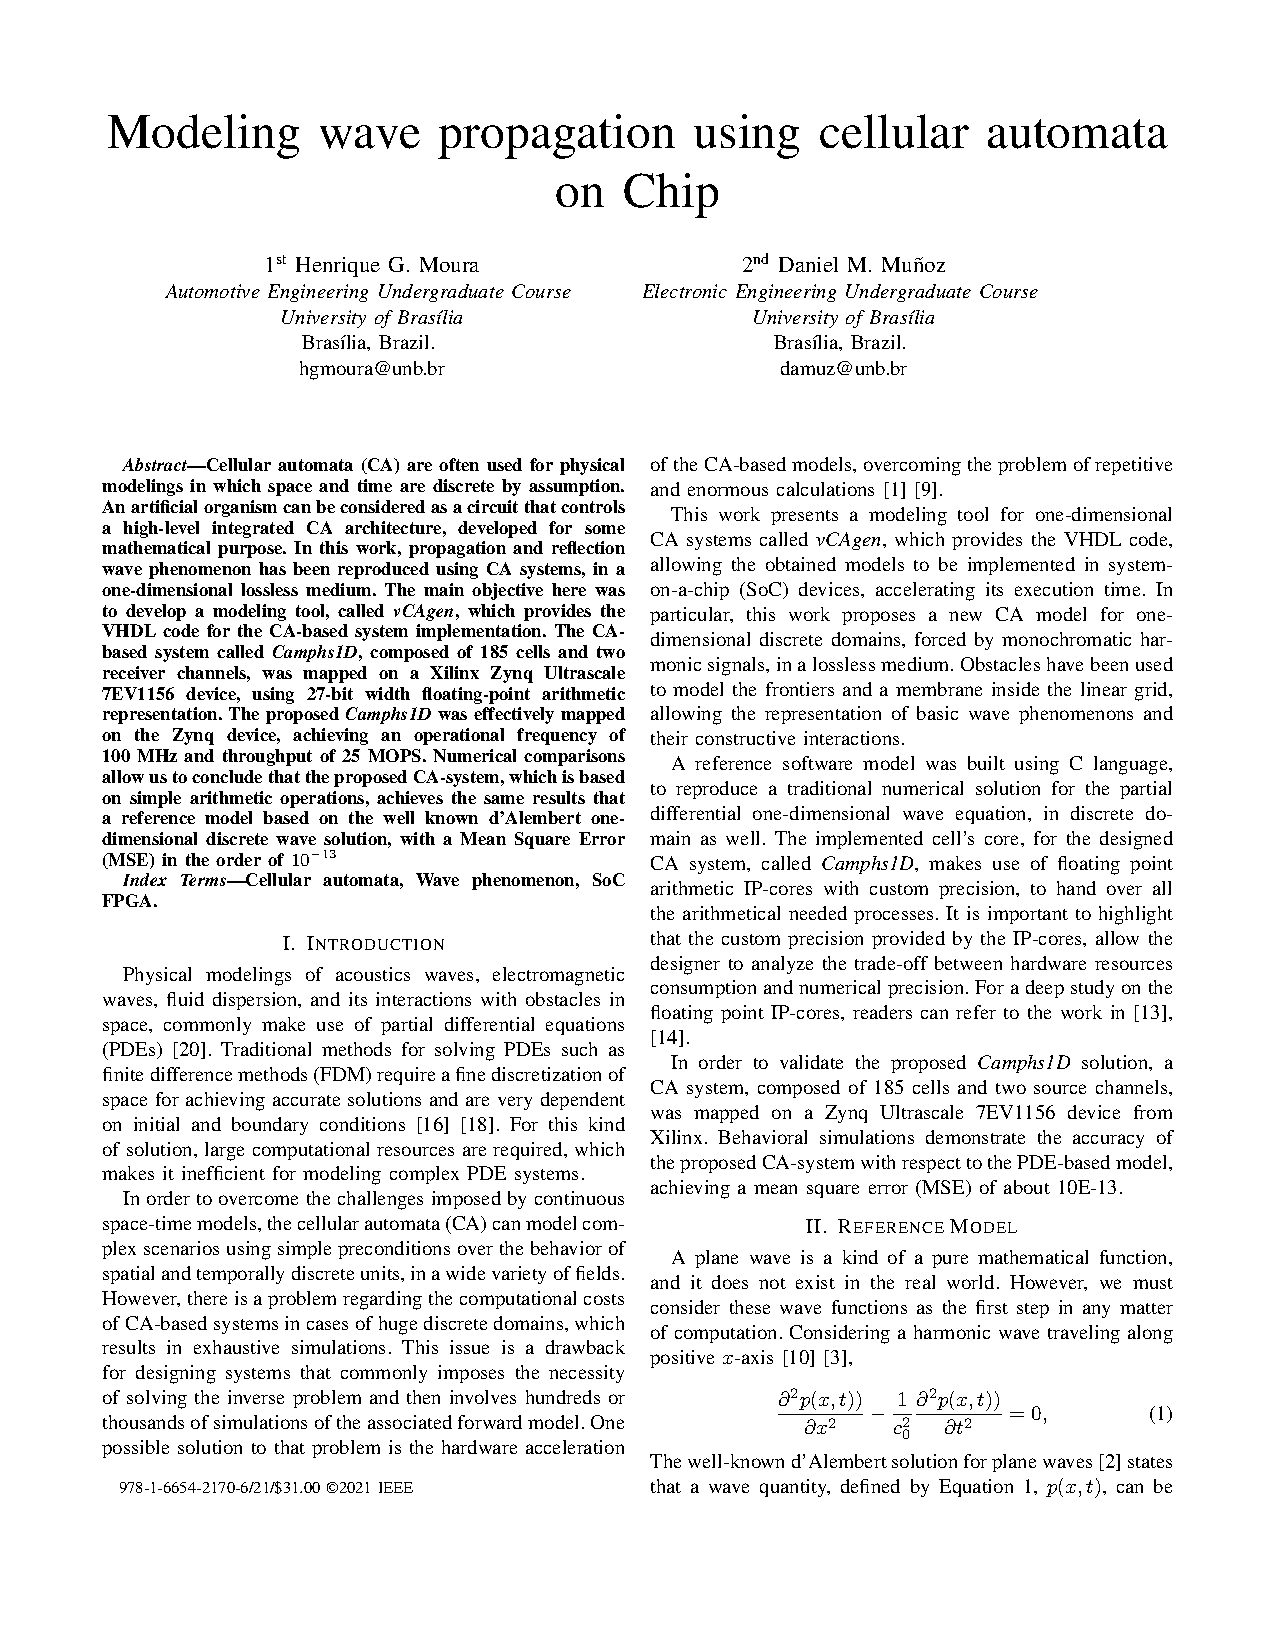
\includepdf[pages=-]{fixos/artigo.pdf}

\end{apendicesenv}
%\begin{anexosenv}

\partanexos

\chapter{Primeiro Anexo}

Texto do primeiro anexo.

\chapter{Segundo Anexo}

Texto do segundo anexo.

\end{anexosenv}


\printindex

\end{document}

